% Gemini生成
\section{引言}
\label{sec:intro}
\begin{figure*}[t]
    \centering
    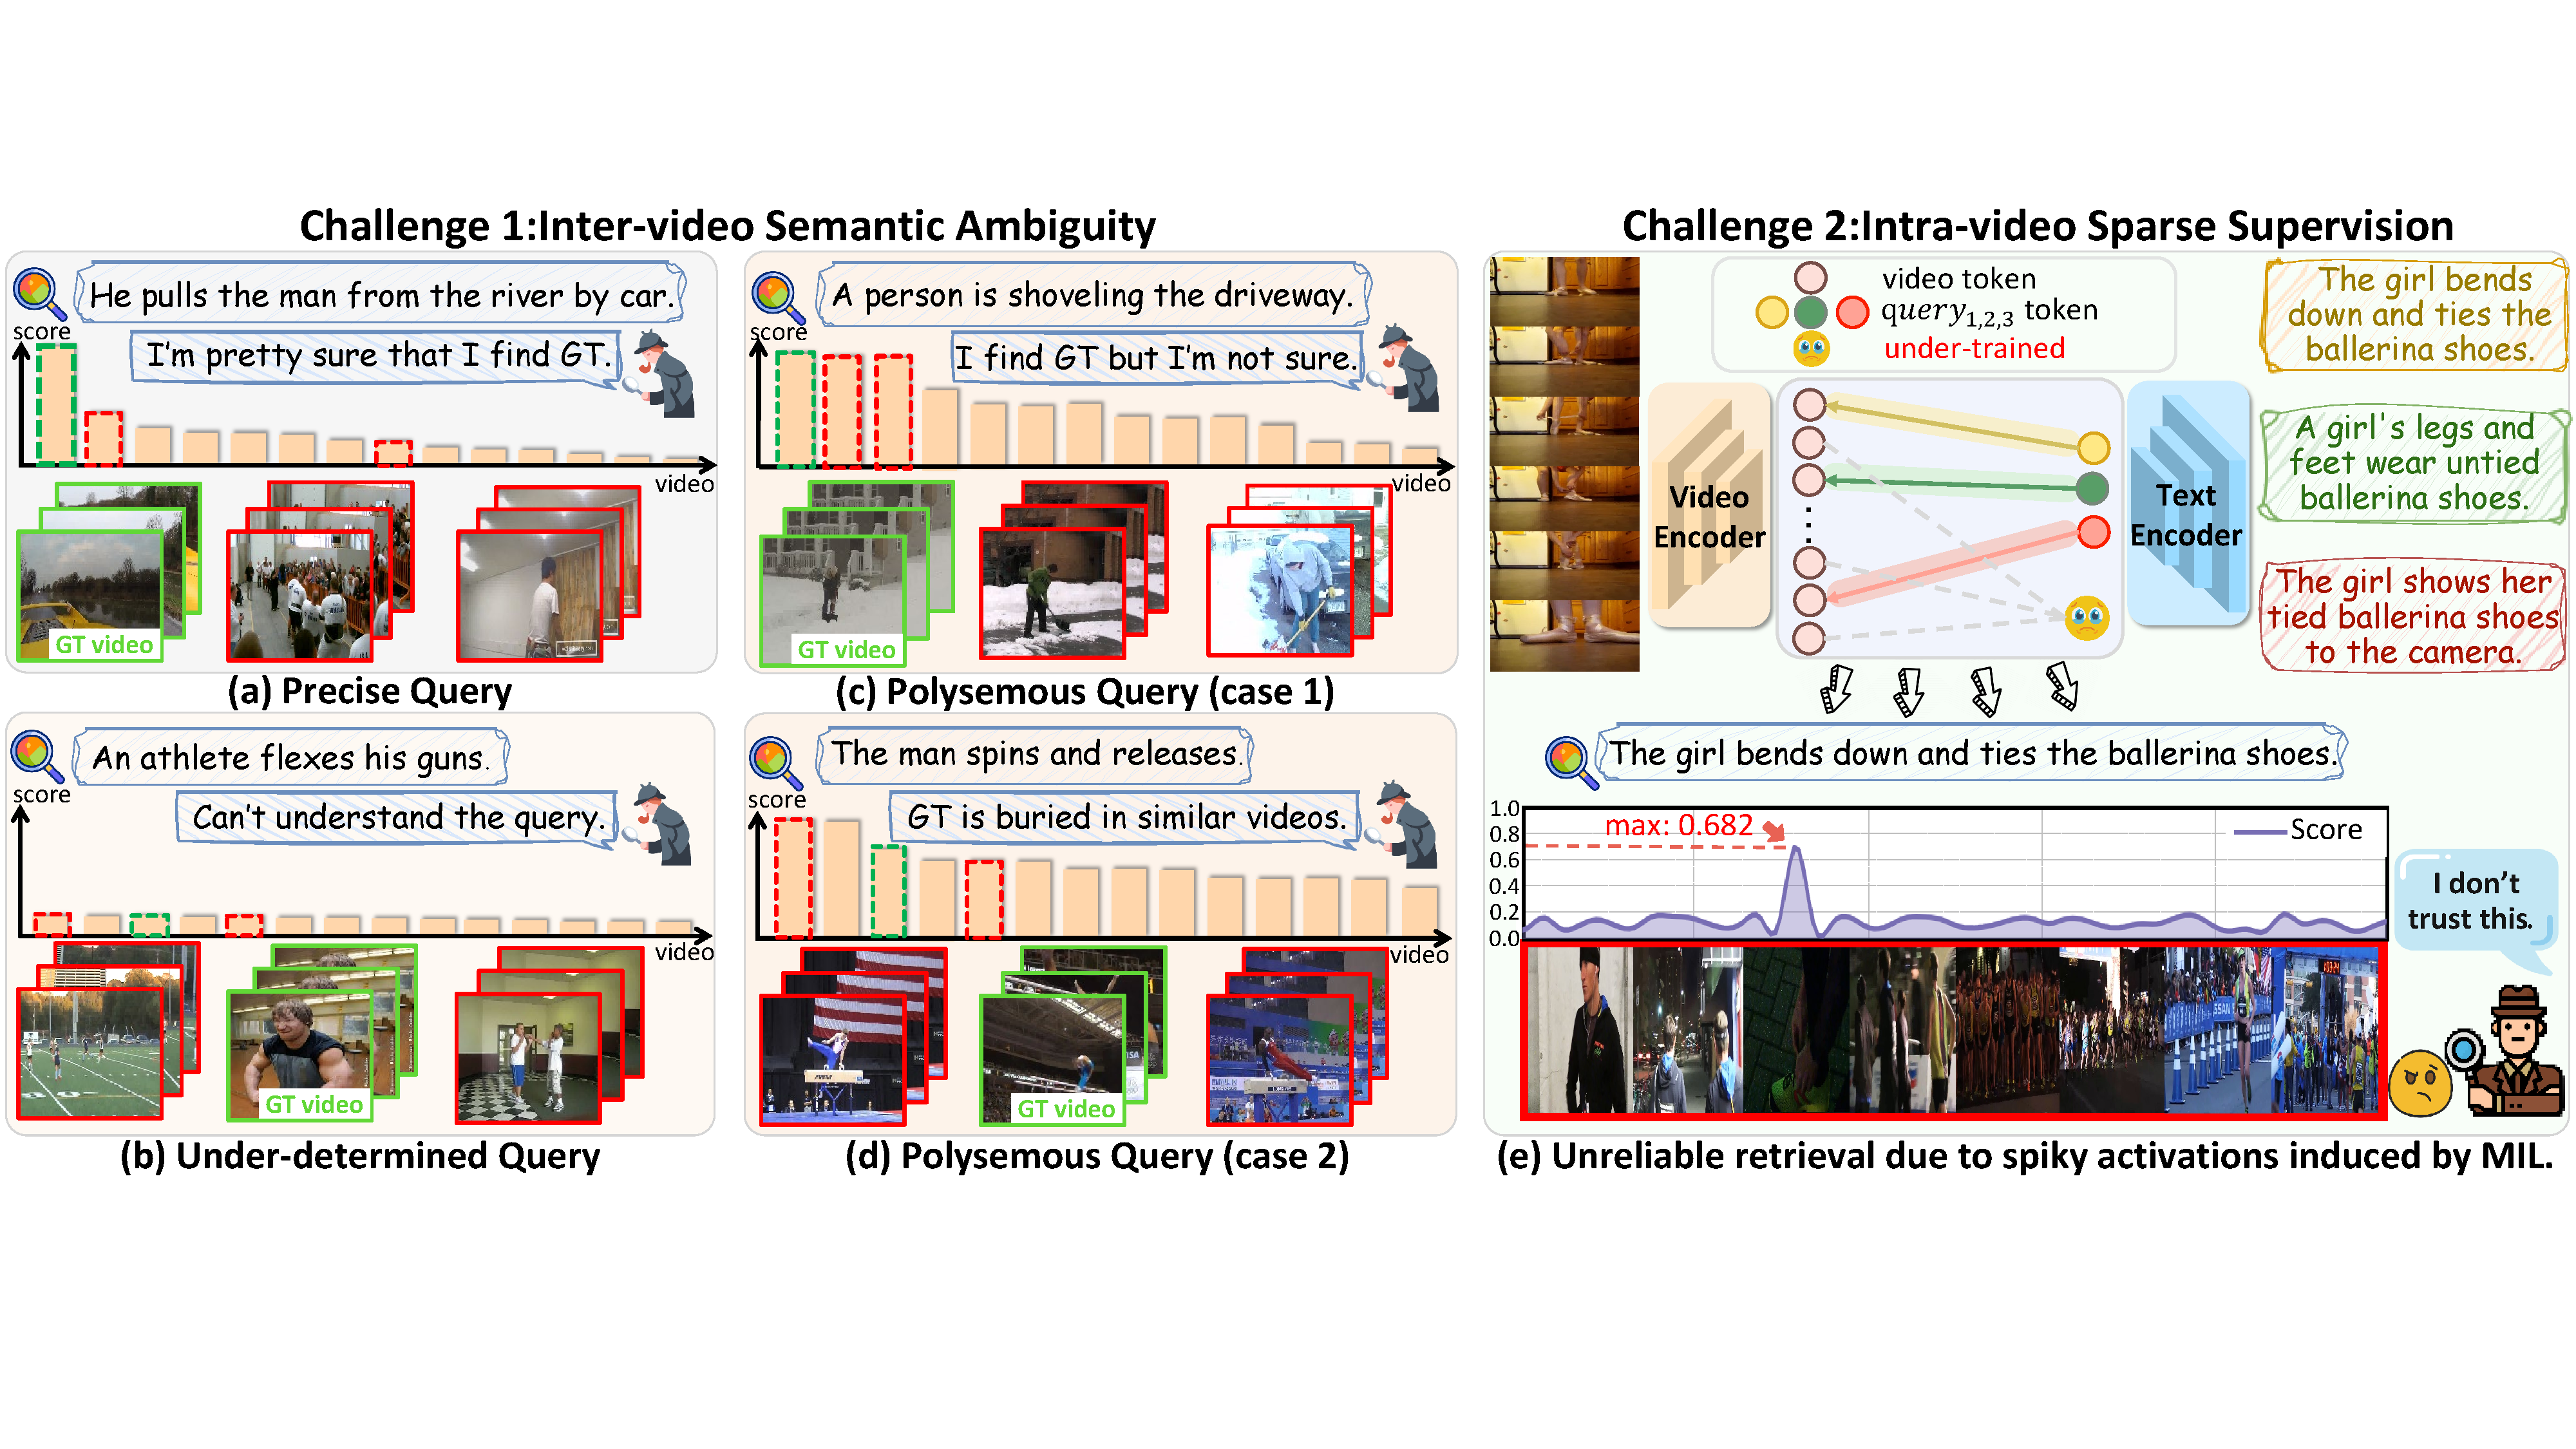
\includegraphics[width=\textwidth]{images/introv3.pdf}
    \caption{(a) \emph{精确查询}产生明显的响应间隔，真实匹配视频的得分显著高于其余候选。
    (b) \emph{信息不足查询}难以被模型正确理解，导致相似度响应较弱，缺乏区分度。
    (c-d) \emph{多义查询}存在语义歧义，对应多个合理候选，需要\emph{进一步甄别}以处理相关不确定性。
    (e) MIL 只优化最相近的配对，造成\emph{监督稀疏}、片段训练不足。模型因而容易受到整体无关的“跑步”视频中的局部噪声干扰，产生虚假尖峰激活，降低检索可靠性。
    }
    \label{fig:Intro}
\end{figure*}

随着在线视频快速增长，文本到视频检索（T2VR）\cite{PIG}受到越来越多关注。大多数 T2VR 方法针对预先裁剪的视频和能够完整描述视频的查询而设计，难以直接对应现实场景。现实中的视频通常未经裁剪，查询也往往只对应其中某些片段。因此，研究者提出了\emph{部分相关视频检索}（PRVR）\cite{ms-sl}，旨在根据描述部分内容的查询检索未经裁剪的视频。
这项任务的根本难点在于数据不对称。与内容丰富的视频相比，文本查询往往简短而含糊，检索过程因此具有内在的不确定性。

对此类不确定性建模需要同时解决视频间与视频内两个层面相互叠加的困难：
(\textbf{i}) \textbf{视频间语义歧义。} 由于内在的不确定性，查询之间常存在细粒度差异。\cref{fig:Intro}(a-d) 表明，除理想的\emph{精确查询}外，真实数据还包含\emph{信息不足查询}（语义信息不足、置信度低）和\emph{多义查询}（语义具有歧义、可以匹配多个候选）。多数既有方法忽略了这种差异\cite{GMMFORMER}，或借助正则化进行隐式处理\cite{RAL,msc-prvr}。ARL\cite{ARL}尝试识别存在歧义的视频与文本配对，但缺少显式量化具体不确定性类型的机制。
(\textbf{ii}) \textbf{视频内监督稀疏。} 视频内部缺少可靠证据，也会加剧视频间歧义。常用的多实例学习（MIL）范式只监督最匹配的单个片段，导致\emph{监督稀疏}。如\cref{fig:Intro}(e) 所示，监督失衡限制了训练信号，使模型难以学习整体表征，容易被虚假的局部噪声干扰。虽然从 CLIP\cite{CLIP} 蒸馏线索可以缓解稀疏性\cite{DL-DKD}，但帧级线索过于零散，无法捕捉确认视频相关性所需的时序变化，进而加剧视频间不确定性，影响检索表现。


为解决上述问题，我们认为模型需要在确定性的相似度分数之外，进一步评估预测的不确定性。本文提出统一的证据学习框架 \modelname{}，在两个层面区分并建模不确定性。
首先，为处理\textbf{视频间不确定性}，我们将跨模态相似度视为证据，并用 Dirichlet 分布进行参数化。由此，模型可以在计算匹配分数的基础上\emph{诊断}查询类型。我们提出不确定性引导识别（UGI）策略，依据\emph{认知不确定性}、\emph{标签一致性}与\emph{偶然不确定性}三项原则对查询分类，并进行查询自适应的标签校准。
其次，为缓解会加剧不确定性的\textbf{视频内监督稀疏}问题，我们试图积累更密集的证据。我们制定灵活最优传输（FOT）方案，在查询与多个相关片段之间建立软对齐。为提高抗噪能力，我们引入\emph{回收槽}吸收无关片段，从而提供更加全面、可靠的时序监督。

我们在 ActivityNet Captions\cite{krishna2017dense}、Charades-STA\cite{gao2017tall} 和 TVR\cite{lei2020tvr} 上开展了大量实验，结果表明 \modelname{} 达到当前先进水平。在标准检索指标之外，进一步分析表明，\modelname{} 能够有效解释查询歧义，并抑制 MIL 中的虚假激活。

本文的主要贡献如下：
\vspace{-.2cm}
\begin{itemize}
    \item[$\bullet$] \emph{\textbf{概念层面}}：我们从不确定性的角度重新审视 PRVR，明确联系了视频间语义歧义和视频内监督稀疏。 \vspace{-.2cm}
    \item[$\bullet$] \emph{\textbf{方法层面}}：我们提出双层证据学习框架 \modelname{}，通过三项判别原则实现细粒度的查询识别和标签校准，再用灵活最优传输构建密集、稳健的时序对齐。\vspace{-.2cm}
    \item[$\bullet$] \emph{\textbf{实验层面}}：\modelname{} 在三个基准上均取得了显著提升。细致的消融研究还验证了它量化查询不确定性以及抑制虚假局部噪声的能力。
\end{itemize}